\chapter{Introduction}
This is a citation \autocite{juliani2018unity}!
\begin{figure}
    \centering
    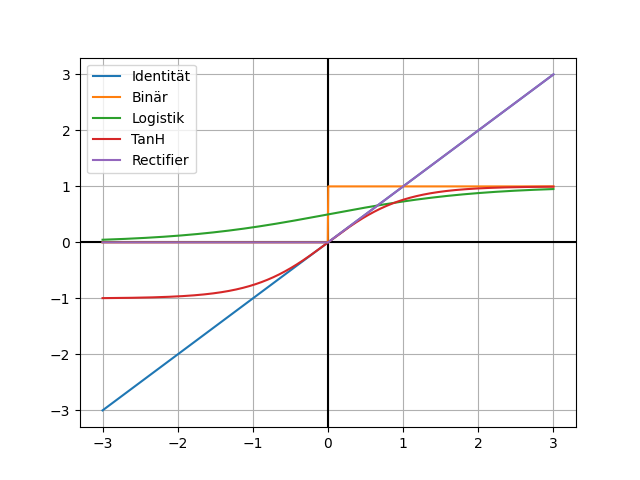
\includegraphics[width=0.8\textwidth]{img/test.png}
    \caption{Einige typische Aktivierungsfunktionen}
    \label{fig:actfn}
\end{figure}

\begin{figure}
    \centering
    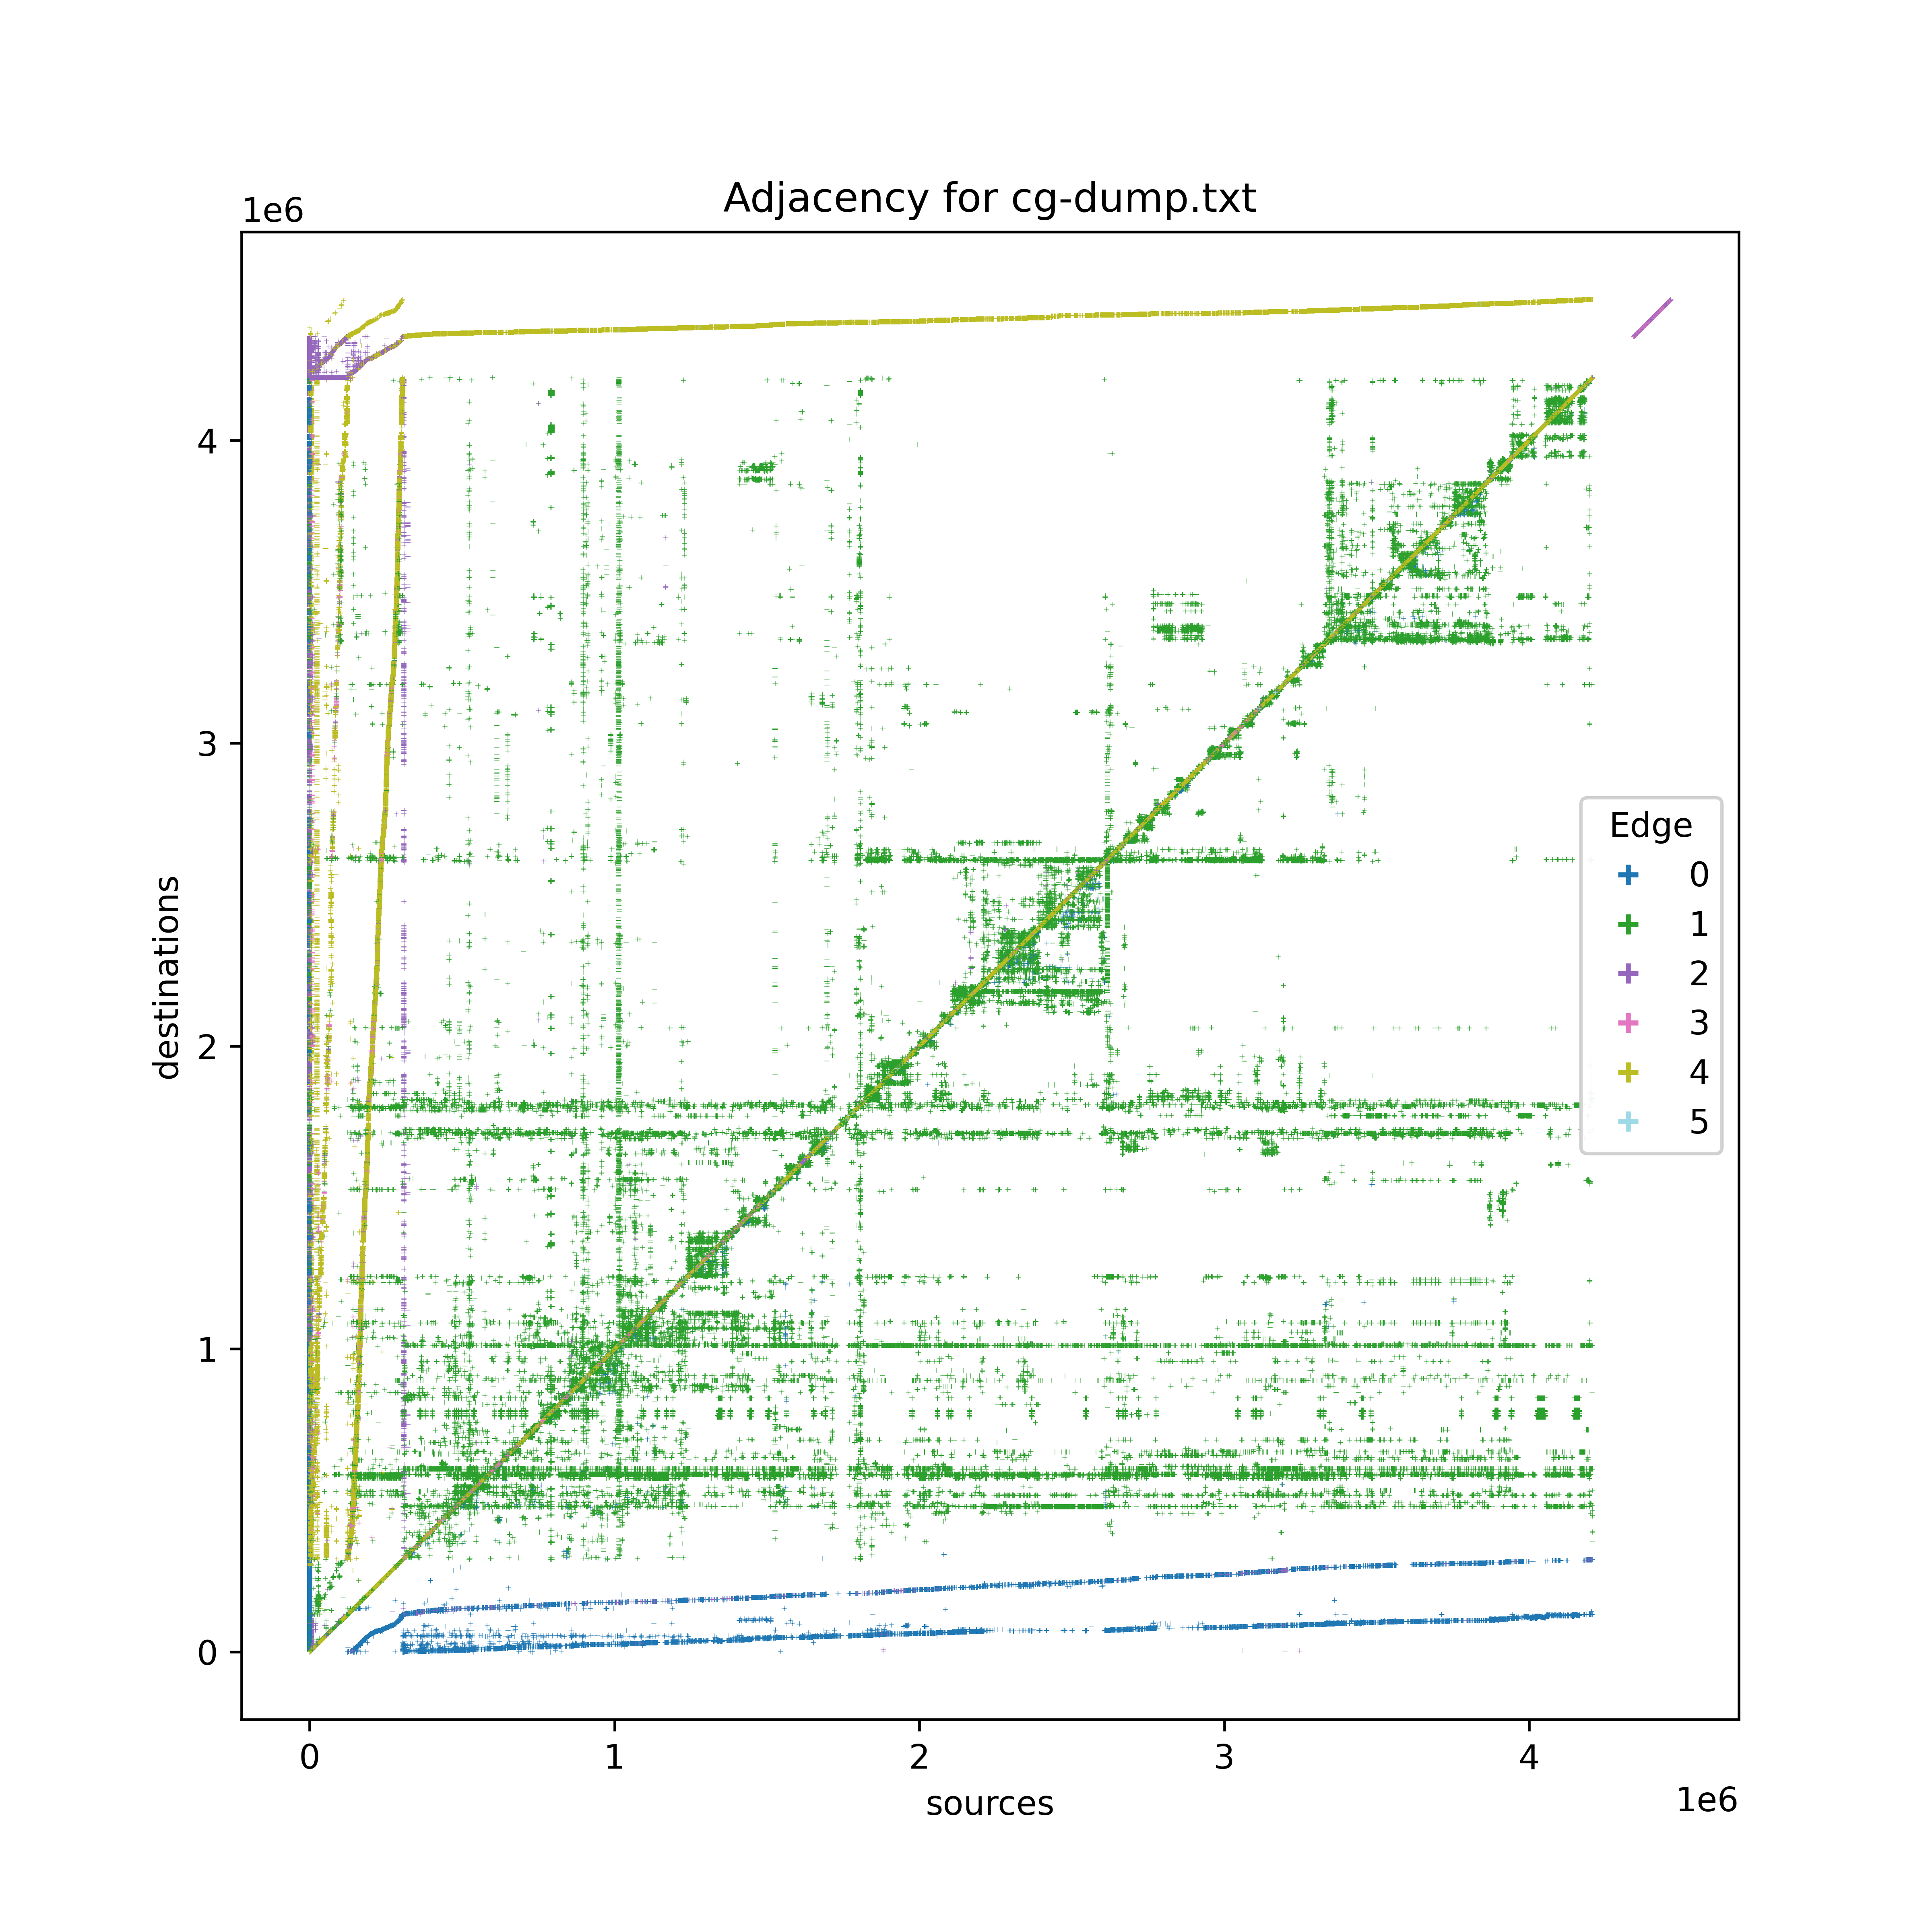
\includegraphics[width=1.\textwidth]{img/linux-consg.png}
    \caption{Adjacency Plot for the Constraint Graph of the Linux Kernel}
    \label{fig:linux-consg}
\end{figure}

\begin{minted}[mathescape, linenos]{python}

    # Note: $\pi=\lim_{n\to\infty}\frac{P_n}{d}$
    title = "Hello World"

    sum = 0
    for i in range(10):
     sum += i
\end{minted}



\begin{table}[h!]
    \begin{center}
        \caption{More rows.}
        \label{tab:table1}
        \begin{tabular}{l|S|r}
            \textbf{Value 1} & \textbf{Value 2} & \textbf{Value 3} \\
            $\alpha$         & $\beta$          & $\gamma$         \\
            \hline
            1                & 1110.1           & a                \\
            2                & 10.1             & b                \\
            3                & 23.113231        & c                \\
            4                & 25.113231        & d                \\ % <-- added row here
        \end{tabular}
    \end{center}
\end{table}


\section{Structure of this Thesis}
\section{Pointer Analysis}
\subsubsection{Steengards Analysis}
\subsubsection{Andersens Analysis}
\subsubsection{Wave Propagation}
\section{Motivation}
\subsection{Static Analysis in Software Development}
\section{Related Work}
\subsection{Context Free Languages}
\subsection{Sequential Analyses}
\subsubsection{SVF}
\subsection{GPU Accelerated Analyses}
\subsubsection{Graspan}
